\documentclass[sigconf]{acmart}
\usepackage{algorithm}
\usepackage{algpseudocode}

% \setcopyright{acmcopyright}
% \copyrightyear{2023}

\begin{document}

%% -------------------

\title{Parallel Feed Forward Calculation of ANNs with CUDA}

\author{Philipp Reinig}
\email{reinig@ovgu.de}
\affiliation{%
  \institution{Otto-von-Guericke University}
  \streetaddress{Universitätsplatz 12}
  \city{Magdeburg}
  \state{Saxony-Anhalt}
  \country{Germany}
  \postcode{39104}
}

%% -------------------

\begin{abstract}
ANNs are a popular method in the field of artificial intelligence. For large networks, the feed forward calculation takes a long time
because the underlying matrix multiplications have a runtime complexity of $O(n^3$). Parallelization is one solution to address this issue.
This paper presents an algorithm for parallel matrix multiplication, analyses it's performance and discusses when it makes sense to apply it.
It was found that a parallel implementation of the matrix multiplication drastically reduces the execution time for large layer sizes $(>1000)$, but
for smaller sizes, the serial implementation is quicker. 
The recommendation is therefore to use both a serial and parallel algorithm for matrix multiplcation during the feed forward calculation and choose dynamically
based on the sizes of the current and next layer.

\end{abstract}

\maketitle

\keywords{neural networks, matrix multiplication, cuda}

\section{Introduction}
Artificial neural networks (ANNs) have increased in popularity in the field of artifical intelligence in recent years.
They are able to find connections in huge data sets and make predictions based on them. 
Large Language Models (LLMs) are special ANNs, which are able to generate human-like text.
They are currently the most promising method in the field of natural language processing.
LLMs like GPT-4 by OpenAI or Bard by Google consist of many billion parameters to achieve their impressive results.
However, large ANNs increase the computational cost for training and feed forward calculations.
The underlying mathematical operations are matrix multiplications with runtime complexity \begin{math}O(n^3)\end{math}.
Therefore parallelization is essential to run the feed forward calculations for large ANNs.
This paper outlines an algorithm for parallel feed forward calculations with CUDA. 

\section{Feed Forward Calculation}{
The feed forward calculation describes the process of calculating
the outputs of an ANN given a certain input vector.
Each node's value is calculated by the dot product of the last layer's node values and the weights of this node.


% \begin{itemize}
%     \item{test}
%     \item{test}
%     \item{test}
% \end{itemize}

\begin{figure}[H]
    % \centering
    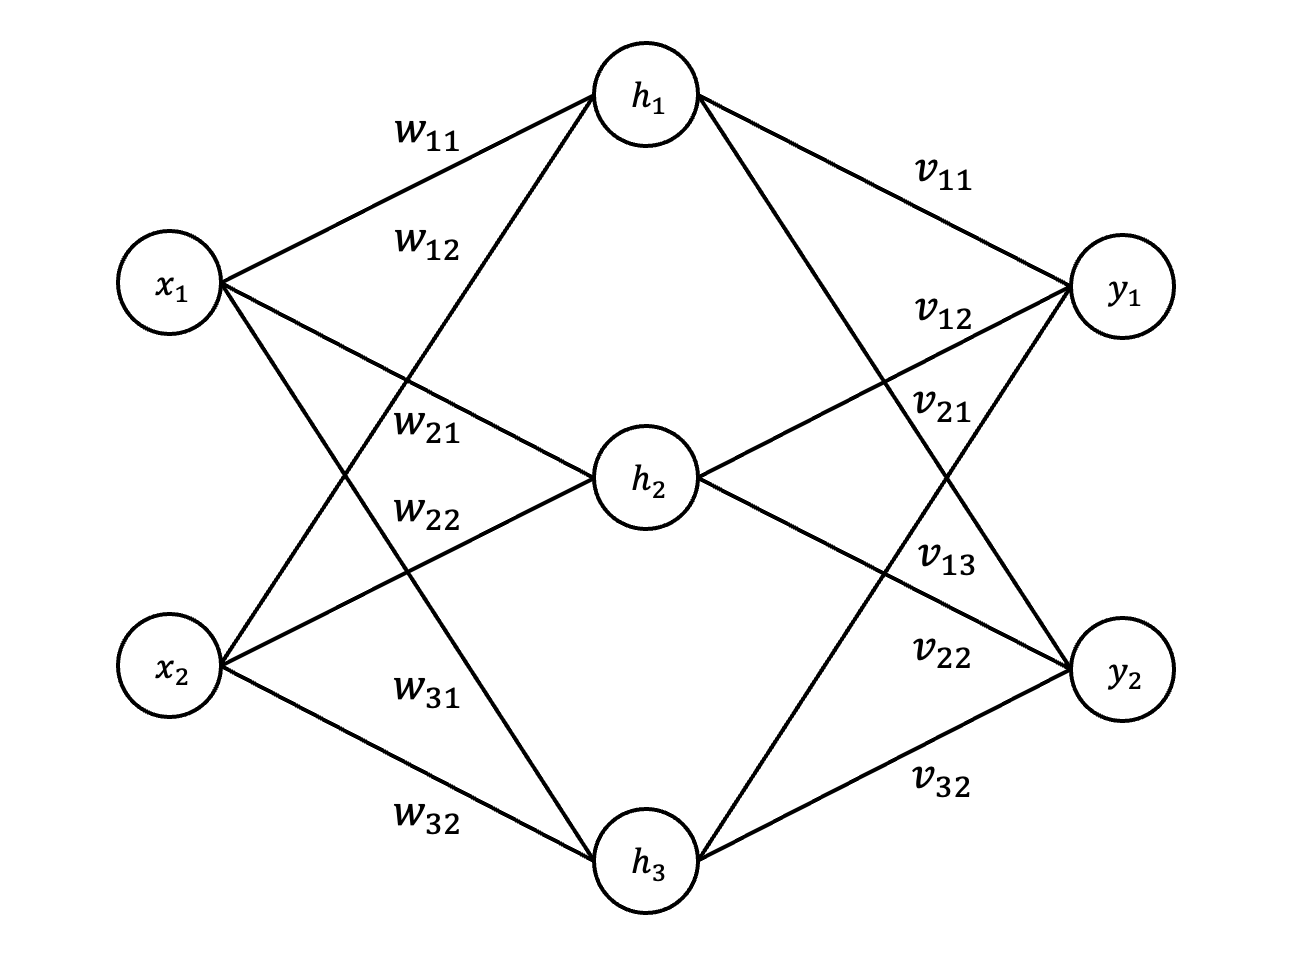
\includegraphics[width=\columnwidth]{imgs/ann_example.png}
    \Description{Example of an ANN with 1 hidden layer}
    \caption{Example of an ANN with 1 hidden layer}
\end{figure}
%\subsection{Matrix representation}
Instead of calculating each node's value one by one, it's also possible to compute an entire layer
by calculating a matrix multiplication.
If one stores each layer's values and all weights in a matrix, the entire state of the ANN is represented by matrices
and the feed forward calculation problem reduces to $n-1$ matrix multiplications for an ANN with $n$ layers.
For the example ANN of Figure 1, the matrix multiplications are:
\begin{displaymath}
\begin{bmatrix}
    h_1 \\
    h_2 \\
    h_3
\end{bmatrix}
^T =
\begin{bmatrix}
    x_1 \\ x_2
\end{bmatrix} ^ T 
*
\begin{bmatrix}
    w_{11} & w_{21} & w_{31} \\
    w_{12} & w_{22} & w_{32}
\end{bmatrix}
\end{displaymath}
\begin{displaymath}
\begin{bmatrix}
    y_{1} \\
    y_{2}
\end{bmatrix}^T = 
\begin{bmatrix}
    h_1 \\
    h_2 \\
    h_3
\end{bmatrix}^T *
\begin{bmatrix}
    v_{11} & v_{21} \\
    v_{12} & v_{22} \\
    v_{13} & v_{32}
\end{bmatrix}
\end{displaymath}

Therefore optimizing and parallelizing of the feed forward calculation reduces to optimizing and
parallelizing matrix multiplication.
}

\section{Optimization and Parallelization}
\subsection{Efficient Algorithms}
First of all, one should decide on an algorithm which is efficient, but most importantly, it has to be well suited to be parallelized.

The standard algorithm for matrix multiplication consists of three nested for loops which is a runtime complexity of $O(n^3)$.

\begin{algorithm}
    \caption{Trivial Matrix Multiplication}
    \begin{algorithmic}[1]
    \Procedure{MatrixMultiplication}{$A, B$}
        \State $n \gets$ number of rows in $A$
        \State $m \gets$ number of columns in $A$
        \State $o \gets$ number of columns in $B$
        \State Let $C$ be a new matrix $n \times o$ matrix of zeros
        \For{$i \gets 1$ to $n$}
            \For{$j \gets 1$ to $m$}
                \For{$k \gets 1$ to $o$}
                    \State $C_{i,j} \gets C_{i,j} + A_{i,k} * B_{k,j}$
                \EndFor
            \EndFor
        \EndFor
        \State \Return{$C$}
    \EndProcedure
    \end{algorithmic}
\end{algorithm}
    

There is the recursive Strassen Algorithm which reduces the runtime complexity from $O(n^3)$ to $O(n^{log_2(7)})\approx O(n^{2,8074})$.
However, it only works with square matrices and in the case of matrix multiplications for the feed forward calculation the first
operand matrix only consists of a single row. 
Therefore, the Strassen Algorithm is not applicable. This issue can be fixed by adding $m-1$ rows to the $1xm$ matrix
containing just 0 values so the amount of rows and columns both equal $m$. This approach also increases the result matrix from
$1$ to $m$ rows, of which $m-1$ rows contain just 0 values. These $m-1$ rows have to be sliced 
to obtain a matrix with the correct dimensions for the next iteration of the feed foward calculation.
In summary, this means calculating $m-1 * x$ unnecessary values to benefit from the slightly better runtime complexity,
where $x$ is the amount of columns of the first operand matrix.
This comparison hasn't been analysed in detail, because it's highly hardware dependent, but regarded highly unlikely that the Strassen algorithm provides an advantage.
The other issue with this algorithm for feed forward calculations is, that it only works with matrices of the same size.
This can be fixed using the same idea just explained, but further increases the amount of unnecessary zero value calculations.

All other ideas available to optimize matrix multiplication are based on partitioning the matrices into blocks, like Fox's method and Cannon's method.
However, they all face the same issues just described and are therefore all regarded unsuitable for the feed forward calculation.

Because of that, the only possibility for this case is parallelizing the trivial matrix multiplication algorithm.

\subsection{Parallelization}
It is possible to parallelize any of the three nested loops of the trivial matrix multiplication algorithm.
Because a GPU is a highly parallelized processor with many thousands of threads running in parallel, it makes 
most sense to devide the computation into the smallest possible portions. This means parallelizing all three of
the nested for loops.
\

\begin{algorithm}[]
    \caption{Matrix Multiplication parallelized with CUDA (worker)}
    \begin{algorithmic}[2]
    \Procedure{MatrixMultiplication}{$A*, B*, C*$}
        \State{$tid \gets$ thread id}
        \State{$row \gets$ tid / A.cols}
        \State{$col \gets$ tid \% A.cols}
        \For{$k \gets 1$ to $B.cols$}
                \State{$C_{row,col} \gets C_{row,col} + A_{1,i} * B_{i,col}$}
        \EndFor
    \EndProcedure
    \end{algorithmic}
\end{algorithm}

\subsection{Results}


The serial and parallel implementations were compared for a neural network consisting of 5 hidden layers so 7 layers in total and different sizes of the layers.

Figure 2 shows a comparison between the runtime of the serial and the parallel implementation. For small layers $(<1000)$, the serial implementation 
is faster. However, the serial implementation scales linearly with the size of the matrices, whereas the parallel implementation has constant runtime if the
amount of necessary threads is less than the amount of streaming multiprocessors available on the GPU * 1024. If the matrix sizes exceed that point, the execution time
scales sublinearly. The advantage of the parallel implementation is higher the bigger the size of the matrices become.
It's therefore advised, to use both variants depending on the size of the matrix to obtain the lowest execution time.
Unfortunately, it was not possible to test the parallel execution time for larger matrix sizes because the global memory of the GPU on the testing machine isn't enough.

\begin{figure}[H]
    % \centering
    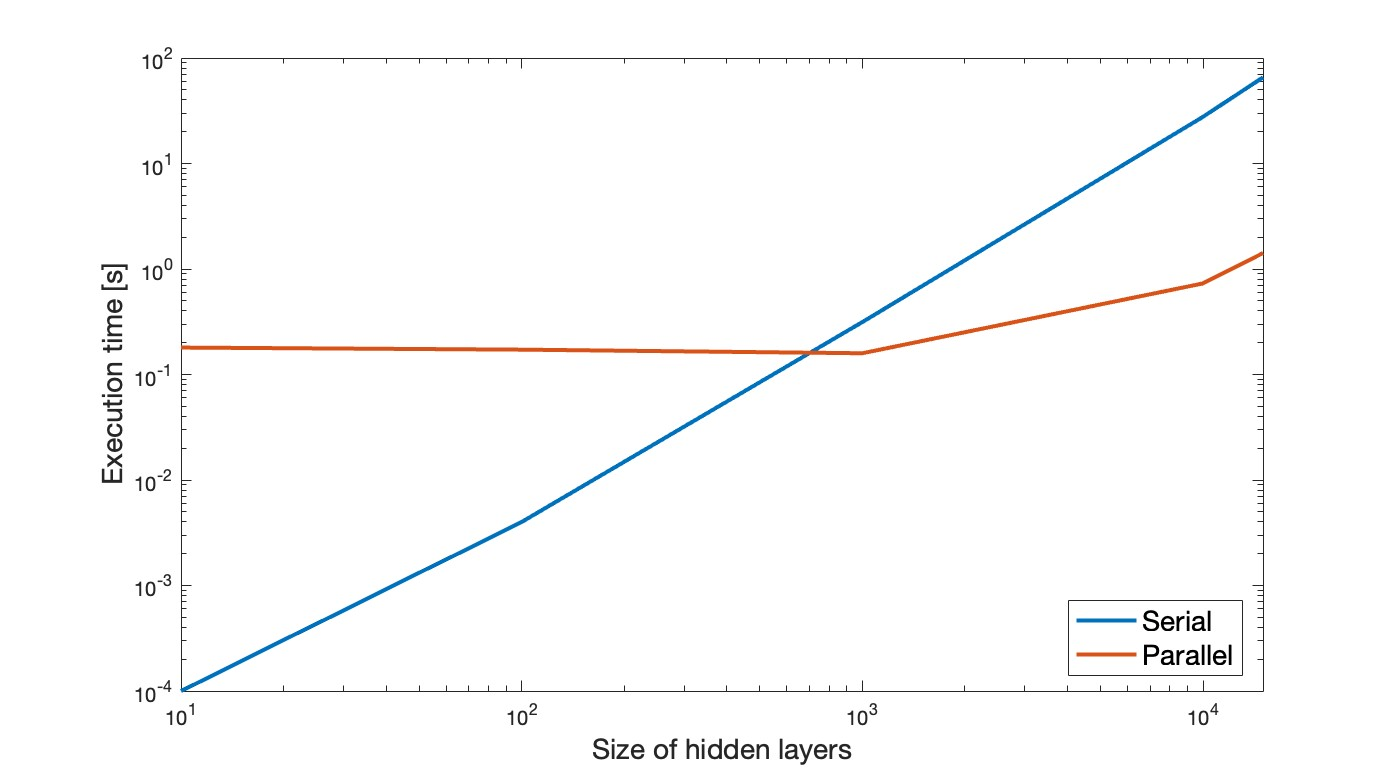
\includegraphics[width=\columnwidth]{imgs/results.jpg}
    \Description{Comparison serial vs parallel implementation}
    \caption{Comparison serial vs. parallel implementation}
\end{figure}

\subsection{Possible improvements}

\begin{itemize}
    \item{The parallel implementation could be improved by further increasing the amount of threads used per matrix multiplication by also parallelising the last for loop.}
    \item{Storing the value of the first operand matrix in shared memory}
    \item{Using the tensor cores available in modern Nvidia GPUs}
\end{itemize}


\section{Summary}
Parallelizing the feed forward calculation of ANNs is necessary to quickly calculate the output values for large layer sizes.
Unfortunately more efficient matrix multiplication algorithms are not suited in the case of the feed forward calculation. Thus one has to parallelize the trivial
matrix multiplication algorithm.
It was shown, that a parallel implementation drastically improves the execution time for large layer sizes of the ANN.
One should keep in mind that the execution time of the serial implementation is faster for small layer sizes. Therefore it's recommended to choose one of the two algorithms dynamically
based on the sizes of the layers to compute the current feed forward iteration.

\end{document}

